En este apéndice se realizará una estimación, tanto del coste como de la planificación del trabajo durante el período de desarrollo, con el objetivo de simular la valoración y presupuesto de un proyecto real en el ámbito laboral.

\section*{Estimación del presupuesto del proyecto}

Haremos un presupuesto del proyecto, en el que incluiremos las horas dedicadas a cada tema estudiado y realizaremos una estimación a precio 7 euros/hora. El análisis del presupuesto se puede observar en la Tabla \ref{tab:estcostes}.

Para facilitar la estimación de los costes, hemos dividido el trabajo en tres partes:

\begin{itemize}
    \item \textbf{Parte teórica}: recoge las tareas relacionadas con el análisis y el estudio de los conceptos de carácter teórico contenidos en el trabajo. Incluiremos la formalización de las nociones básicas para el proyecto y el desarrollo de las demostraciones matemáticas.
    \item \textbf{Parte práctica}: reúne las prácticas relacionadas con la programación, análisis y validación de los experimentos. Además tendremos en cuenta el equipo utilizado y los tiempos dedicados a instalación de bibliotecas y software empleados.
    \item \textbf{Parte general}: agrupa las labores de elaboración de la memoria y reuniones con los tutores (presencial u online).
\end{itemize}

El cómputo total es de 8.047 euros. Teniendo en cuenta que el período de trabajo útil ha sido de aproximadamente 5 meses, el sueldo medio mensual equivale a 1.609 euros brutos. Para un trabajador sin experiencia, este valor es bastante fiel a la realidad.

\section*{Planificación del trabajo}

El diseño de la planificación se ha realizado con el software \href{https://www.ganttproject.biz}{GanttProject}, que es un programa de código abierto utilizado para administrar proyectos, pudiendo usar entre otras muchas herramientas, un diagrama de Gantt. Para el desarrollo de la planificación, hemos usado la misma división en partes que la presentada en la sección anterior.

En la planificación original nos habría gustado presentar el trabajo para la convocatoria de septiembre, pero debido a algunos problemas derivados de la carga docente a lo largo del curso 2020-2021 y a la concreción de los experimentos asociados al proyecto, se ha acabado retrasando hasta el mes de noviembre.

Además es destacable, si comparamos las Figuras \ref{fig:planning_prev} y \ref{fig:planning}, que el tiempo dedicado tanto al estudio como la formalización de las diferentes medidas de equidad, ha sido mayor al previsto inicialmente.\\

\begin{figure}[h]
	\centering
	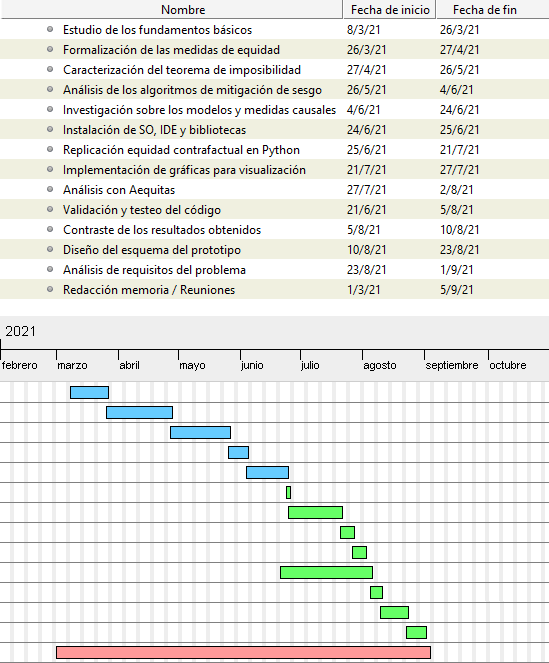
\includegraphics[width=12.7cm]{planificacion_prev.png}
	\caption{Planificación original del desarrollo del trabajo.}
    \label{fig:planning_prev}
\end{figure}

\clearpage

En ambos casos, la parte general es una tarea que se desarrolla a lo largo del período de trabajo, ya que la redacción de la memoria y las tutorías se realizan de forma simultánea al análisis teórico y práctico del proyecto. 

En la planificación final, hemos establecido el mes de abril como inicio del proyecto. Además el periodo de exámenes de junio también ralentizó en gran medida el avance del proyecto propuesto. Todos estos factores se pueden intuir observando la Figura \ref{fig:planning}, donde indicamos en color azul la parte teórica, en verde la parte práctica y en rojo la parte general.\\

\begin{figure}[h]
	\centering
	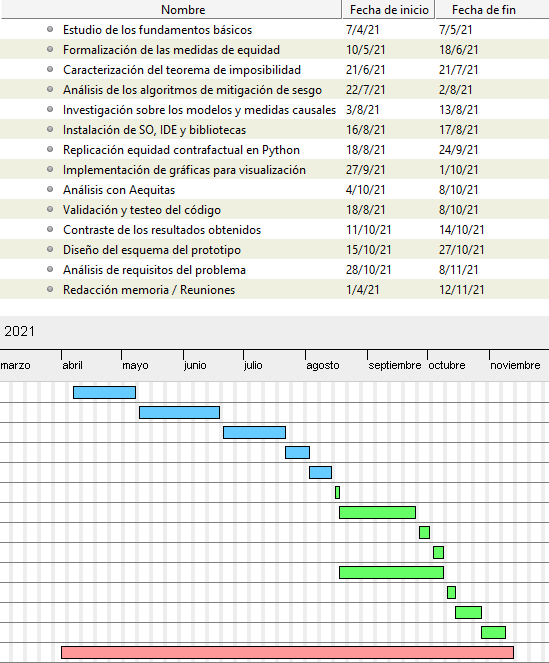
\includegraphics[width=12.7cm]{planificacion.png}
	\caption{Planificación final del desarrollo del trabajo.}
    \label{fig:planning}
\end{figure}

\begin{table}[h]
\centering
\resizebox{13.8cm}{!} {
\begin{tabular}{lccc}
\hline
\multicolumn{1}{c}{\textbf{Concepto}}                                                         & \begin{tabular}[c]{@{}c@{}}\textbf{Tiempo}\\ \textit{(horas)}\end{tabular} & \begin{tabular}[c]{@{}c@{}}\textbf{Coste} \\ \textit{(euros/hora)}\end{tabular} & \begin{tabular}[c]{@{}c@{}}\textbf{Coste total}\\ \textit{(euros)}\end{tabular} \\ \hline
\textbf{Parte general}                                                                        & \multicolumn{1}{l}{}                                     & \multicolumn{1}{l}{}                                         & \multicolumn{1}{l}{}                                          \\ \hline
Redacción de la memoria                                                                       & 300                                                      & 7                                                         & 2.100                                                            \\
Reuniones con los tutores                                                                     & 14                                                       &    -                                                        &   -                                                          \\ \hline
\textbf{Parte teórica}                                                                        & \multicolumn{1}{l}{}                                     & \multicolumn{1}{l}{}                                         & \multicolumn{1}{l}{}                                          \\ \hline
Estudio de los fundamentos básicos                                                                & 80                                                      & 7                                                          & 560                                                           \\
\begin{tabular}[c]{@{}l@{}}Formalización de las medidas \\ de equidad\end{tabular}            & 150                                                        & 7                                                          & 1.050                                                            \\
\begin{tabular}[c]{@{}l@{}}Caracterización del teorema \\ de imposibilidad\end{tabular}       & 90                                                       & 7                                                          & 630                                                            \\
\begin{tabular}[c]{@{}l@{}}Análisis de los algoritmos de \\ mitigación de sesgo\end{tabular}  & 32                                                        & 7                                                           & 224                                                           \\
\begin{tabular}[c]{@{}l@{}}Investigación sobre los \\ modelos y medidas causales\end{tabular}     & 45                                                        & 7                                                          & 315                                                           \\ \hline
\textbf{Parte práctica}                                                                       & \multicolumn{1}{l}{}                                     & \multicolumn{1}{l}{}                                         & \multicolumn{1}{l}{}                                          \\ \hline
Equipo de trabajo: ASUS TUF                                                                  &        -                                                 & -                                                           & 949                                                          \\
Instalación de SO, IDE y bibliotecas                                                           & 3                                                        & 7                                                           & 21                                                            \\
\begin{tabular}[c]{@{}l@{}}Replicación de un modelo de \\ equidad contrafactual en Python\end{tabular} & 120                                                        & 7                                                           & 840                                                            \\
\begin{tabular}[c]{@{}l@{}}Implementación de gráficas \\ para visualización\end{tabular}      & 16                                                       & 7                                                          & 112                                                           \\
Análisis con Aequitas                                                          & 28                                                      & 7                                                         & 196                                                           \\
Validación y testeo del código                                                                & 110                                                       & 7                                                          & 770                                                            \\
Contraste de los resultados obtenidos                                                         & 40                                                       & 7                                                          & 280                                                           \\ \hline
\textbf{Cómputo total del proyecto}                                                           & 1.028                                                       &    -                                                        & 8.047                                                           \\ \hline
\end{tabular}
}
\caption{Estimación del coste del proyecto.}
\label{tab:estcostes}
\end{table}